% Online Resource 1. Scientific content: R5; numerical data: R4-frozen-1.
\documentclass[11pt]{article}
\usepackage[margin=1in]{geometry}
\usepackage[authoryear,round]{natbib}
\usepackage{fix-cm}
\usepackage[T1]{fontenc}
\usepackage{microtype,amsmath,amssymb,amsthm,mathtools,bm}
\usepackage{booktabs,array,graphicx,enumitem,tabularx,float,longtable}
\usepackage{url}
\usepackage{hyperref}
\hypersetup{hidelinks}
\setlength{\emergencystretch}{2em}
\newtheorem{theorem}{Theorem}[section]
\newtheorem{proposition}[theorem]{Proposition}
\newtheorem{corollary}[theorem]{Corollary}
\newtheorem{lemma}[theorem]{Lemma}
\theoremstyle{definition}\newtheorem{definition}[theorem]{Definition}
\theoremstyle{remark}\newtheorem{remark}[theorem]{Remark}
\numberwithin{equation}{section}
\newcommand{\R}{\mathbb R}\newcommand{\E}{\mathbb E}\newcommand{\Prob}{\mathbb P}
\newcommand{\norm}[1]{\left\lVert#1\right\rVert}\newcommand{\TV}{\mathrm{TV}}
\newcommand{\dd}{\,\mathrm d}\newcommand{\cA}{c_\alpha}\newcommand{\sg}{\operatorname{sigmoid}}
\newcommand{\sech}{\operatorname{sech}}\newcommand{\Var}{\operatorname{Var}}
\newcommand{\gap}{\operatorname{gap}}\newcommand{\osc}{\operatorname{osc}}
\newcommand{\diag}{\operatorname{diag}}\newcommand{\SA}{\mathrm{S}\alpha\mathrm{S}}
\newcommand{\1}{\mathbf 1}

\setcitestyle{authoryear,round,semicolon,aysep={},yysep={,}}

\hypersetup{pdftitle={Online Resource 1: Score-based Metropolis--Hastings with stable proposals: Invariance and calibration},pdfauthor={Truong Vu}}
\renewcommand{\thesection}{S\arabic{section}}
\renewcommand{\thetable}{S\arabic{table}}
\renewcommand{\thefigure}{S\arabic{figure}}
\title{Online Resource 1\\Supplementary information for\\Score-based Metropolis--Hastings with stable proposals: Invariance and calibration}
\author{Truong Vu\\Departments of Mathematics and Computational Medicine\\
University of California, Los Angeles (UCLA)\\Los Angeles, California, USA\\
Corresponding email: [AUTHOR: supply email]}
\date{Prepared for submission to \emph{Statistics and Computing}}
\begin{document}
\maketitle

\noindent This supplement preserves additional target-modeling, statistical and computational results and gives the full experimental protocol. Sections, equations, theorems, tables and figures prefixed by S belong to this document. Unprefixed section, equation, and theorem numbers refer to the accompanying main article. Bibliographic citations use author--year notation.

\section{Proper graph Gibbs targets and their optimum weights}\label{sec:graphs}
\subsection{Normalize the target before analyzing its sampler}\label{sec:decoder}
The displayed graph models in \citet{fractional} take $u\in\R^N$, bounded energies depending on $\tanh u$ or $\sg(u)$, and a density proportional to $e^{-E(u)/\eta}$. Since the energies are bounded, these functions have infinite integrals on $\R^N$. This prevents a stationary Gibbs-probability interpretation of the displayed formulas; it does not refute finite-time optimization improvements.

A proper replacement defines a Gibbs law on the bounded relaxed cube, then pulls it back to $u$. For MaxCut, with $y=\tanh u$,
\begin{align}
p_\eta(u)&\propto e^{-y^TAy/(2\eta)}\prod_i\sech^2u_i,\label{eq:cutproper}\\
\nabla_u\log p_\eta&=-\eta^{-1}(1-y^2)\odot Ay-2y.
\end{align}
For vertex cover, with $v=\sg(u)$ and a simple unweighted graph,
\begin{equation}
F(v)=\sum_iv_i+\lambda\sum_{(i,j)\in E}(1-v_i)(1-v_j),\qquad \lambda>1,\label{eq:VCenergy}
\end{equation}
use
\begin{align}
p_\eta(u)&\propto e^{-F(v)/\eta}\prod_iv_i(1-v_i),\label{eq:VCproper}\\
\nabla_u\log p_\eta&=-\eta^{-1}v(1-v)\odot[\1-\lambda A(\1-v)]+\1-2v.\label{eq:VCproperscore}
\end{align}
These are changes to the source target, not missing constants that can be ignored. All graph results below concern these explicitly normalized replacements.

Each energy is affine in one coordinate with the others fixed. Replacing coordinates successively by their better endpoints therefore never increases energy. For vertex cover, after endpoint rounding, adding a vertex incident to $j\ge1$ uncovered edges changes $F$ by $1-\lambda j<0$. Thus completion yields a feasible cover whose size is no greater than the starting relaxed energy. It follows that the relaxed minimum is exactly the minimum cover size $k_*$. For MaxCut, the minimum relaxed energy equals the minimum binary energy $|E|-2\operatorname{cut}$. These statements do not say that a sufficiently low relaxed state is easy to obtain.

\paragraph{Coordinatewise decoder.}
Throughout this section, $\operatorname{decode}(v)$ denotes the following vertex-cover procedure. Fix a coordinate permutation, independent of $v$ and $\eta$, and set $z=v$. Visit each coordinate $i$ once in that order and replace $z_i$ by an endpoint in $\{0,1\}$ minimizing $F$ with every other coordinate held at its current value; choose zero in a tie. If an uncovered edge remains after this sweep, add one of its endpoints to the cover and repeat until all edges are covered. Edge and endpoint choices use a fixed measurable deterministic rule, which may depend on the original $v$. Completion adds vertices only and does nothing to an already feasible cover. The results below hold for every fixed coordinate order and such completion rule. They do not cover arbitrary energy-decreasing maps to binary vertices.

\subsection{A sharper finite-temperature concentration bound}
\begin{proposition}[Coordinatewise partition-function lower bound]\label{prop:graphconcentration}
Let $E$ attain its global minimum $E_*$ at a vertex of a cube of side $\ell$, and let $|\partial_iE|\le L_i$. Define
\[
b_i(\eta)=\frac{\eta}{L_i\ell}(1-e^{-L_i\ell/\eta}),
\]
with the continuous convention $b_i=1$ if $L_i=0$. For the Gibbs law relative to uniform cube measure,
\begin{equation}
\Prob_\eta(E-E_*\ge\gamma)\le
\min\left\{1,\frac{e^{-\gamma/\eta}}{\prod_i b_i(\eta)}\right\}.\label{eq:graphconcentration}
\end{equation}
A positive base density $r$ bounded between $r_{\min}$ and $r_{\max}$ adds a factor $r_{\max}/r_{\min}$ on the right.
\end{proposition}
\begin{proof}
In inward coordinates $t_i\in[0,\ell]$ from an optimal vertex, $E-E_*\le\sum_iL_it_i$. Integrating $e^{-\sum_iL_it_i/\eta}$ under the product uniform reference gives the lower bound $\prod_ib_i$ for the partition function after removing $e^{-E_*/\eta}$. The numerator for the event is at most $e^{-\gamma/\eta}$. Bounded-density comparison proves the last statement.
\end{proof}
For energy-decreasing rounding, a nonoptimal unweighted cut requires relaxed energy excess at least two, and a nonminimum feasible cover requires relaxed penalized-energy excess at least one. Thus \eqref{eq:graphconcentration}, with $\gamma=2$ or $1$ respectively, bounds failure to obtain an optimum. A sampler's total-variation error adds to the failure probability. Compared with a small-corner-cube estimate using $\sum_iL_i$, this bound retains the separate coordinate slopes. It still has severe dimension and low-temperature dependence, so it is not a polynomial-time optimization result.

\subsection{Zero-temperature sampling is generally not uniform over optimal covers}
Identify a binary cover $C$ with its indicator vector. Let $\mathcal C_*$ be the set of minimum covers. For $C\in\mathcal C_*$ define the inward slopes
\begin{equation}
a_i(C)=\begin{cases}
1,&i\notin C,\\
\lambda d_{V\setminus C}(i)-1,&i\in C,
\end{cases}
\quad w_C=\prod_i a_i(C)^{-1},\quad W=\sum_{C\in\mathcal C_*}w_C.\label{eq:cornerslopes}
\end{equation}
All slopes are strictly positive. Indeed every member of a minimum cover has a neighbor outside it; otherwise that vertex could be removed.

\begin{theorem}[Corner asymptotics and the first correction]\label{thm:corner}
For the Gibbs law of \eqref{eq:VCenergy} relative to Lebesgue measure on $[0,1]^N$,
\begin{equation}
Z_\eta\sim e^{-k_*/\eta}\eta^N W.\label{eq:graphZ}
\end{equation}
Fix the coordinatewise decoder of Section~\ref{sec:decoder}, with any fixed coordinate order and the stated deterministic tie and completion rules. It returns each fixed $C\in\mathcal C_*$ with limiting probability
\begin{equation}
\Prob_\eta(\operatorname{decode}(v)=C)\longrightarrow w_C/W.\label{eq:cornerweights}
\end{equation}
For the fixed graph and $\lambda>1$, the more precise expansion is
\begin{equation}
\Prob_\eta(\operatorname{decode}(v)=C)
=\frac{w_C}{W}\left[1-\eta(B_C-\overline B)+O(\eta^2)\right],\label{eq:firstordergraph}
\end{equation}
where
\[
B_C=\lambda\sum_{(i,j)\in E}\frac{(1-2C_i)(1-2C_j)}{a_i(C)a_j(C)},
\qquad \overline B=\sum_C(w_C/W)B_C.
\]
\end{theorem}
\begin{proof}
Multiaffinity expresses $F(v)$ as a convex combination of its binary vertex values. If a fractional point minimized $F$, every vertex in its positive-weight coordinate face would also minimize. Such a face contains adjacent binary vertices; two minimum covers cannot differ in just one coordinate, because they have the same cardinality. Hence the minimizers are precisely the finitely many minimum-cover vertices.

In inward coordinates $v_i=C_i+(1-2C_i)t_i$, the exact quadratic expansion is
\[
F(v)=k_*+\sum_i a_i(C)t_i+
\lambda\sum_{(i,j)\in E}(1-2C_i)(1-2C_j)t_it_j.
\]
Choose disjoint sufficiently small corner neighborhoods. Strictly positive inward slopes ensure a bound $F-k_*\ge\frac12\sum_i a_i t_i$ there. Outside their union, compactness and the absence of other minima give a positive energy gap. After setting $t_i=\eta z_i$, dominated convergence on each corner gives the integral $\prod_i\int_0^\infty e^{-a_i z_i}\dd z_i=w_C$, proving \eqref{eq:graphZ}.

For each minimum-cover vertex $C$, continuity and the positive inward slopes give a sufficiently small corner box on which $(1-2C_i)\partial_iF(z)>0$ for every $i$. Coordinate minimization then sets the updated coordinate to $C_i$ and keeps the iterate in the same box. Induction over the fixed order returns $C$ exactly; since $C$ is a cover, completion makes no further change. Thus $\operatorname{decode}$ is locally constant with value $C$ on that box. Contributions from outside the finitely many boxes are exponentially small relative to $e^{-k_*/\eta}\eta^N$, proving \eqref{eq:cornerweights}.

Expand the rescaled quadratic term's exponential to first order. Under the independent exponential laws of rates $a_i$, $\E z_i z_j=1/(a_i a_j)$ for distinct vertices. The corner integral is therefore
$e^{-k_*/\eta}\eta^Nw_C[1-\eta B_C+O(\eta^2)]$.
The remainder is uniformly integrable: on a fixed small corner the quadratic term is bounded in absolute value by a sufficiently small multiple of $\sum_i a_i z_i$ after multiplication by $\eta$, and the second-order remainder is bounded by an integrable polynomial times an exponential with smaller positive rates. The tails outside the rescaled corner are exponentially small. Normalize the finitely many corner integrals to obtain \eqref{eq:firstordergraph}.
\end{proof}
For the four-vertex path and $\lambda=1.7$, the minimum covers are $\{1,3\}$, $\{2,3\}$, and $\{2,4\}$ in one-based labels. Their limiting probabilities are
\begin{equation}
\left(\frac7{38},\frac{12}{19},\frac7{38}\right),\label{eq:pathweights}
\end{equation}
not $(1/3,1/3,1/3)$. The central cover has two inward slopes $0.7$, whereas each other cover has slopes $0.7$ and $2.4$. The central probability equals
$12/19-0.57182430\,\eta+O(\eta^2)$. This is an entropic preference in the continuous relaxation, not a defect in an exact sampler.

\subsection{A computable local base density cancels this preference}
The weights in \eqref{eq:cornerweights} suggest a repair that does not require listing the minimum covers.
\begin{theorem}[Uniform limiting weights without knowing the optima]\label{thm:balancedgraph}
For any fixed $\kappa>0$, define on the relaxed cube
\begin{align}
t_i(v)&=\sum_jA_{ij}(1-v_j),\\
D_i(t)&=(1-\lambda t)^2+\kappa^2\sin^2(\pi t),\\
r(v)&=\prod_i\sqrt{D_i(t_i(v))}.\label{eq:localbase}
\end{align}
Then $r$ is smooth, strictly positive, bounded above and below on $[0,1]^N$, and computable from local graph quantities without identifying any optimum. For the modified target
\begin{equation}
\pi^{\rm bal}_\eta(v)\propto r(v)e^{-F(v)/\eta},\label{eq:balancedtarget}
\end{equation}
the coordinatewise decoder fixed as in Theorem~\ref{thm:corner} returns every minimum cover with probability
\begin{equation}
\Prob^{\rm bal}_\eta(\operatorname{decode}(v)=C)
=\frac1{|\mathcal C_*|}+O(\eta).\label{eq:uniformoptima}
\end{equation}
\end{theorem}
\begin{proof}
A zero of $D_i$ would require both $t=1/\lambda$ and $t$ integer. This is impossible since $0<1/\lambda<1$. Positivity, smoothness, and compactness give the bounds on $r$. At a minimum-cover vertex $C$, every $t_i(C)$ is an integer. If $i\notin C$, all its neighbors are in $C$, so $t_i(C)=0$; if $i\in C$, $t_i(C)=d_{V\setminus C}(i)\ge1$. Thus
\[
r(C)=\prod_i|1-\lambda t_i(C)|=\prod_i a_i(C)=w_C^{-1}.
\]
The corner expansion with a smooth base multiplies each leading corner weight by $r(C)$. All become one. The same coordinatewise decoder is locally constant at each minimum-cover vertex by the proof of Theorem~\ref{thm:corner}. Its corner probabilities therefore have uniform leading weights, with an order-$\eta$ remainder from the smooth-base expansion, proving \eqref{eq:uniformoptima}.
\end{proof}
The added score is explicit. Write
$D_i'(t)=-2\lambda(1-\lambda t)+\kappa^2\pi\sin(2\pi t)$; then
\begin{equation}
\nabla_v\log r=-\tfrac12 A^T\left(D_i'(t_i)/D_i(t_i)\right)_{i=1}^N.\label{eq:basescore}
\end{equation}
Under $v=\sg(u)$ multiply this by $v(1-v)$ and add it to the score in \eqref{eq:VCproperscore}. The finite-temperature target is explicitly changed. This theorem supplies no claim of efficient mixing on arbitrary graphs, and a comparable MaxCut result needs separate treatment when flat directions occur.

\subsection{An oracle reference sampler for checking the asymptotics}
For a small graph whose optima can be enumerated, form an independence proposal by choosing $C\in\mathcal C_*$ with weights $w_C/W$, then drawing independent inward coordinates $t_i\in[0,1]$ from truncated exponentials of rates $a_i(C)/\eta$. For the balanced target use uniform component weights. The resulting finite mixture has an explicit density and full support, so independence MH is exact for the respective cube target.

The corner proof also shows $\norm{q_\eta-\pi_\eta}_{\TV}=O(\eta)$: on each corner both laws have the same leading product-exponential density and an integrable order-$\eta$ correction; outside the corners both have exponentially small mass. For independent $X\sim\pi_\eta$, $Y\sim q_\eta$, the stationary mean rejection equals
$\norm{\pi_\eta\otimes q_\eta-q_\eta\otimes\pi_\eta}_{\TV}\le2\norm{\pi_\eta-q_\eta}_{\TV}$.
Thus acceptance is $1-O(\eta)$. This is a useful numerical reference but not a general optimization algorithm: the \emph{reference proposal} knows the optima. In contrast, the local base \eqref{eq:localbase} does not.


\subsection{Numerical validation on the four-vertex path}
For the four-vertex path, $\lambda=1.7$, and local-base parameter $\kappa=1$, tensor Gauss--Legendre quadrature and independent oracle-mixture MH agree at the three low temperatures in Table~\ref{tab:graph}. The archived decoder visits coordinates in order $1,2,3,4$ and chooses zero on an endpoint tie. Completion scans edges in path order, adds the endpoint with the larger original relaxed coordinate, and chooses the lower-index endpoint on a tie. This is the coordinatewise decoder of Section~\ref{sec:decoder}; no code or numerical result is changed. The decoded central-cover probabilities are conditional on returning an optimum; the quadrature optimum probability differs from one only at negligible numerical scale for these temperatures, and all sampled decoded covers in the corresponding low-temperature runs were optimal.

For this path, the derivative bounds in Proposition~\ref{prop:graphconcentration} may be chosen as $(L_1,L_2,L_3,L_4)=(1,2.4,2.4,1)$. A nonminimum decoded cover requires $F-k_*\ge1$, so \eqref{eq:graphconcentration} bounds its probability without using zero observed failures. For the balanced base with $\kappa=1$, $r_{\max}\le13.52$ and $r_{\min}\ge0.4^4$: if $|1-1.7t|<0.4$, then $t\in(6/17,14/17)\subset(1/6,5/6)$ and $\sin^2(\pi t)\ge1/4$; otherwise the squared linear term is at least $0.16$. Thus $r_{\max}/r_{\min}\le528.125$. At the largest displayed temperature $0.02$, the resulting failure bounds are less than $7.0\times10^{-15}$ for the original base and $3.7\times10^{-12}$ for the balanced base, and decrease at the other two temperatures. The conditional/unconditional probability difference for any particular optimum is no greater than this failure probability.

\begin{table}[!htbp]\centering\small
\caption{Central minimum-cover probability for the path graph. Quadrature references use 96 nodes per coordinate and were compared with 64 nodes.}
\begin{tabular}{@{}rrrrr@{}}\toprule
$\eta$ & Original-base quadrature & Original-base MH & Balanced quadrature & Balanced MH\\\midrule
0.020 &0.620481&$0.620895\pm0.000319$&0.347279&$0.347514\pm0.000274$\\
0.010 &0.625967&$0.626519\pm0.000312$&0.339649&$0.339830\pm0.000272$\\
0.005 &0.628749&$0.629351\pm0.000297$&0.336294&$0.336454\pm0.000235$\\\midrule
Limit &0.631579&$12/19$&0.333333&$1/3$\\\bottomrule
\end{tabular}\label{tab:graph}
\end{table}
For the original base, the 64-versus-96-node central-probability difference is below $1.9\times10^{-9}$ at $\eta=0.02$ and below $4\times10^{-13}$ at $\eta=0.01$. At $\eta=0.005$, the first-order prediction from \eqref{eq:firstordergraph} is $0.628720$, compared with quadrature $0.628749$. These are convergence checks, not interval-arithmetic proofs. At the higher temperatures $0.1$ and $0.2$, the discontinuous decoding indicators were not sufficiently resolved by this quadrature sequence. Those values are retained in the data but are \emph{not} treated as accurate reference probabilities.

For the original base, oracle-MH acceptance increases from $0.94708$ at $\eta=0.02$ to $0.98711$ at $\eta=0.005$. With the balancing base it increases from $0.96300$ to $0.99159$. This is consistent with the proved $1-O(\eta)$ oracle acceptance behavior. It does not demonstrate an efficient solver on unknown large instances: the validation proposal uses the enumerated optima, whereas the local base itself does not.

\begin{figure}[!htbp]\centering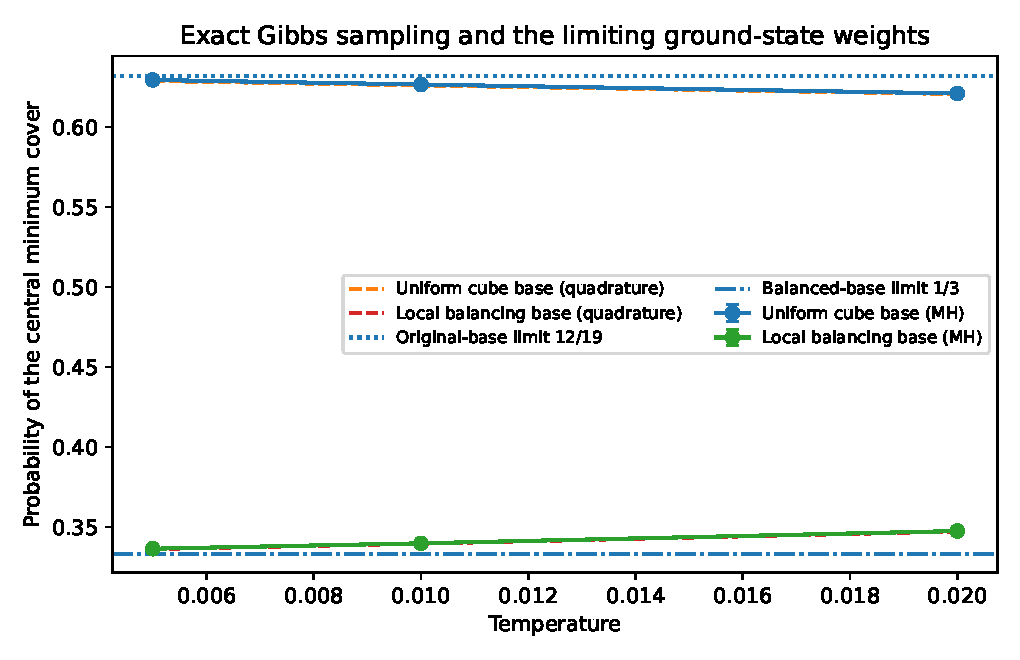
\includegraphics[width=.86\linewidth]{figures/final_graph_weights.pdf}
\caption{Continuous-relaxation entropic weights and their local cancellation. Only temperatures with checked quadrature convergence are plotted as reference values.}
\label{fig:graph}
\end{figure}


\section{Finite-variance score learning and certified acceptance}\label{sec:statistical}
\subsection{Ordinary stable scores: finite-variance supervision and exact risk}
\begin{proposition}[A statistically well-posed score label]\label{prop:label}
For (1.5), put $T=-\xi/(2S)$. Then
\begin{equation}
\E[T\mid\xi=z]=\nabla\log f_\alpha(z),\qquad
\E\norm T^2=\frac d2\Gamma(1+2/\alpha).\label{eq:scorelabel}
\end{equation}
More generally, for every $p>0$,
\begin{equation}
\E\norm T^p=
\frac{\Gamma((d+p)/2)}{\Gamma(d/2)}
\frac{\Gamma(p/\alpha)}{\beta\Gamma(p/2)}<\infty.\label{eq:labelmoments}
\end{equation}
\end{proposition}
\begin{proof}
Differentiate the conditional Gaussian mixture; its conditional score is $-z/(2s)$, so the conditional-expectation identity follows after division by the marginal density. For $\varphi_s(z)=(4\pi s)^{-d/2}\exp(-\|z\|^2/(4s))$,
\[
 \sup_z\|\nabla\varphi_s(z)\|
 \le (4\pi)^{-d/2}(2\mathrm e)^{-1/2}s^{-(d+1)/2}.
\]
The inverse moment $\mathbb E S^{-(d+1)/2}$ is finite, so differentiation under the mixture follows by domination; the density itself is dominated by $(4\pi S)^{-d/2}$. For $r>0$, Tonelli and the Laplace transform give
\[
\E S^{-r}=\frac1{\Gamma(r)}\int_0^\infty t^{r-1}e^{-t^\beta}\dd t
=\frac{\Gamma(r/\beta)}{\beta\Gamma(r)}.
\]
Since $T=-Z/\sqrt{2S}$, multiplying this expression at $r=p/2$ by the Gaussian norm moment proves \eqref{eq:labelmoments} and \eqref{eq:scorelabel}.
\end{proof}
Thus the input has infinite variance when $\alpha<2$, but the score label has all finite moments. Any nonzero linear proxy of $\xi$ has infinite moments of order at least $\alpha$, unlike the true score. Regressing $T$ on $\xi$ estimates the ordinary, not fractional, score.

For an explicit finite-sample result in one dimension, partition the unit stable law into $m$ known equal-probability bins $B_j$. Let $s_m$ be the piecewise-constant $L^2(f_\alpha)$ projection of the true score, with values $\theta_j=\E[T\mid\xi\in B_j]$. The bin probabilities are known exactly; this is not the usual estimator that divides by a random bin count. Given $n$ iid labels, define
\[
\widehat\theta_j=\frac mn\sum_{i=1}^nT_i\1_{\xi_i\in B_j},
\qquad \widehat s_m=\sum_j\widehat\theta_j\1_{B_j}.
\]
\begin{theorem}[Exact finite-sample histogram risk]\label{thm:risk}
\begin{equation}
\E\norm{\widehat s_m-s_\alpha}_{L^2(f_\alpha)}^2
=\norm{s_m-s_\alpha}_{L^2(f_\alpha)}^2+
\frac{m\E T^2-\norm{s_m}_{L^2(f_\alpha)}^2}{n}.\label{eq:risk}
\end{equation}
For nested refining bins, $m\to\infty$ and $m/n\to0$ imply $L^2$ consistency. If bin endpoints are $b_j$, the exact projection values used for validation are $\theta_j=m[f_\alpha(b_j)-f_\alpha(b_{j-1})]$.
\end{theorem}
\begin{proof}
Each coefficient is unbiased. Its variance is
$m^2\Var(T\1_{B_j})/n$. Multiply by the bin mass $1/m$ and sum. The result is $(m\E T^2-\sum_j\theta_j^2/m)/n$. Orthogonality of $s_m$ and the projection residual gives \eqref{eq:risk}. Conditional-expectation convergence proves the approximation term tends to zero for nested partitions generating the Borel sigma field. The endpoint formula follows from integrating $s_\alpha f_\alpha=f_\alpha'$ on a bin.
\end{proof}
The numerical risk experiment measures the estimation part relative to $s_m$, not the approximation term relative to the full score. This one-dimensional theorem is not a neural generalization bound in arbitrary dimension. A learned unit score must be scaled as $h^{-1}\widehat s_m((y-x-\tau b(x))/h)$, and reverse-proposal coverage still matters.

\subsection{Certified acceptance: almost sure termination versus finite mean work}
Exact target scores determine a log ratio by
\begin{equation}
\log p(y)-\log p(x)=\int_0^1s(x+t(y-x))^T(y-x)\dd t.\label{eq:scoreintegral}
\end{equation}
This is an established score-integration approach \citep{sjoberg}, also used in Appendix~A.4.2 of \citet{fractional}. Valid enclosures for this integral give valid enclosures for the log Hastings ratio. One fixed uniform variable is drawn; enclosures are refined until they determine whether $\log U<G$. Shrinking enclosures give almost-sure termination in exact arithmetic, but not automatically finite expected work.

\begin{theorem}[Expected-work threshold for certified refinement]\label{thm:work}
Suppose dyadic quadrature levels $n=1,2,4,\ldots$ have a valid error bound $Bn^{-p}$ for the log ratio, and total work through level $n$ is at most a constant times $n$. For fixed proposal endpoints, if $p>1$,
\begin{equation}
\E[\mathrm{work}\mid x,y]\le C_p(1+B^{1/p}).\label{eq:work}
\end{equation}
For $p=1$, finite mean work is not guaranteed even when termination is almost sure and the enclosure centers equal the exact answer.
\end{theorem}
\begin{proof}
The density of $\log U$ on $(-\infty,0)$ is at most one. The probability that a level-$n$ enclosure of half-width $Bn^{-p}$ remains undecided is therefore at most $\min(1,2Bn^{-p})$. Bound the expected work by the dyadic sum of each level cost times the probability of reaching it. Split the sum at $n\asymp B^{1/p}$. The low-level sum is $O(1+B^{1/p})$ and the remaining geometric series converges exactly when $p>1$.

For the counterexample take a true log ratio $G=-1$, exact enclosure centers at every level, and half-width $B/n$. Choose a refinement implementation whose additional work at each level is bounded above and below by positive constants times $n$. At sufficiently large $n$, the probability of remaining undecided is asymptotic to $2e^{-1}B/n$. The next level then costs order $n$, giving a positive constant contribution at every level and infinite mean total work. Equality with $\log U$ has probability zero, so termination still occurs almost surely.
\end{proof}
If a quadrature rule of order $p$ has a valid bound $B\le C\norm{y-x}^{p+1}$, then \eqref{eq:work} is integrable over stable displacements provided $1+1/p<\alpha$ and the drift part has the same required moment. For example, $p=2$ suffices under these assumptions when $\alpha>3/2$, and $p=4$ when $\alpha>5/4$. This is a sufficient condition, not a lower complexity bound for every algorithm. It requires the corresponding derivative bounds. Floating-point code needs roundoff-aware enclosures to be formally certified; ordinary numerical agreement is not such a certificate. An arbitrary nonconservative learned score field does not define the intended target ratio in \eqref{eq:scoreintegral}.


\subsection{Numerical checks of score risk and refinement work}
The ordinary-score histogram experiment uses equal stable-probability bins and simulated labels from Proposition~\ref{prop:label}. For $\alpha=1.5$ and $m=64$, Table~\ref{tab:scorerisk} reports estimation risk relative to the exact histogram projection; it does not include approximation error relative to the full score. The observed estimation risks follow the exact $m/n$ variance law within observed sampling variation. Additional bin counts 16 and 256 and stability indices 1.2 and 1.8 are included in the raw results.
\begin{table}[!htbp]\centering
\caption{Score-label regression: 32 independent training replicates. The approximation error of the histogram relative to the full score is not included in this table.}\label{tab:scorerisk}
\begin{tabular}{@{}rrr@{}}\toprule
$n$ & Observed estimation risk & Exact expected estimation risk\\\midrule
1,000 &$0.038682\pm0.001565$&0.037673\\
10,000 &$0.004068\pm0.000185$&0.003767\\
100,000 &$0.000352\pm0.000013$&0.000377\\\bottomrule
\end{tabular}
\end{table}

The certified-work test uses $G=-1$, exact enclosure centers, half-width $n^{-p}$, and two million independent uniforms. The expected work truncated at the maximum panel count grows from about 7.23 at cap 16 to 30.77 at cap $2^{20}$ for $p=1$. For $p=2$ and $p=4$ it stabilizes near 4.209 and 2.940. This directly tests the refinement mechanism of Theorem~\ref{thm:work}; it is not a claim about the evaluation cost of an arbitrary learned score network.


\section{Implementation and verification details}\label{sec:repro}
\subsection{Stable generation and exact projection}
The primary simulations generate the positive stable scale by the Kanter transformation \citep{kanter}. For independent $U\sim\operatorname{Unif}(0,\pi)$ and $E\sim\operatorname{Exp}(1)$,
\begin{equation}
S=\frac{\sin(\beta U)}{(\sin U)^{1/\beta}}
\left(\frac{\sin((1-\beta)U)}{E}\right)^{(1-\beta)/\beta},
\qquad 0<\beta<1.
\end{equation}
The implementation evaluates its logarithm before exponentiation and raises an error rather than clipping a nonfinite state or scale. The Gaussian endpoint uses $S=1$. The independent scalar replication in Section~5.9 instead uses the symmetric Chambers--Mallows--Stuck transformation \citep{cms},
\begin{equation}
\xi=\frac{\sin(\alpha U)}{(\cos U)^{1/\alpha}}
\left(\frac{\cos((1-\alpha)U)}{E}\right)^{(1-\alpha)/\alpha},
\quad U\sim\operatorname{Unif}(-\pi/2,\pi/2).
\end{equation}
Both conventions have characteristic function $\exp(-|t|^\alpha)$ in one dimension.

For the projection in (5.1), condition on the current remaining vector $x_\perp$ and write its Gaussian increment as $Z_\parallel e+Z_\perp$, where $e=x_\perp/\|x_\perp\|$ when $x_\perp\ne0$. The orthogonal Gaussian components are independent, and $\|Z_\perp\|^2$ is chi-square with $d-2$ degrees of freedom. Squaring the proposed vector gives (5.1). At $x_\perp=0$ any fixed direction may be used, giving the same distribution. Conditional on the shared scale, all dependence of the target and acceptance ratio on the other coordinates is through their squared radius. Hence this is an exact lumped Markov chain for the reported observables, not an approximation to their joint law. It cannot be used to claim the runtime of updating or storing full $d$-dimensional vectors.

\subsection{Autocorrelation estimates and seed conventions}
For a retained array with time in rows and independent chains in columns, the implementation subtracts each chain's sample mean, computes its autocovariances by an FFT, divides lag-$k$ products by the number of available pairs, and pools across chains. Adjacent autocorrelation pairs starting with lags zero and one are retained until the first nonpositive pair and monotonized by successive minima. The reported integrated autocorrelation estimate is $-1$ plus twice their sum, with a lower truncation at one. This is an initial-positive monotone-sequence diagnostic based on \citet{geyer}. Its reversible-chain justification is not automatically available for the nonreversible proxy chains; there it is only a descriptive finite-run calculation. Finite trajectory length and centering can underestimate a very long correlation time. The long-run replacements at dimensions 256 and 4096 are therefore explicit in the data, plot-finalization code and table-export script.

Each reported standard error is the sample standard deviation of the independent replicate-level statistic divided by the square root of the number of replicates. Reuse of seeds across different parameter configurations creates comparisons with shared randomness, not additional independent replicates within one configuration. The scripts record all seeds. The principal formula-validation scale batches use seeds $6{,}192{,}200+100i+r$ for stability-index position $i$ and replicate $r$. Neural initialization and training-pair generators use seeds $510{,}034+r$ and $522{,}900+r$; the frozen-network chain uses $749{,}489+r$. Long projected checks use $710{,}000+r$. Fresh scalar-generator replications use $931{,}022+r$.

\subsection{Historical record map}
The separately supplied \texttt{stable\_score\_historical\_diagnostics.zip} contains the original \texttt{archive/code/} directory, numerical records, selected trajectories and network weights. These are preserved bytes, not data reconstructed from printed tables. The release map identifies the source archive and each retained file by SHA256. Historical scripts are for reproducing those specific experiments, not the active guarded posterior API.

\begin{table}[tb]\centering\footnotesize
\caption{Historical numerical sources. Paths are relative to the named historical package's \texttt{archive/code/}; JSON files are in \texttt{results/}. The machine-readable map supplies exact hashes and table/figure labels.}\label{tab:files}
\begin{tabular}{p{.29\linewidth}p{.64\linewidth}}\toprule Experiment & Script and principal record\\\midrule
Acceptance and shells & \texttt{analytic\_experiments.py}; \texttt{acceptance\_scaling.json}, \texttt{shell\_separation.json}\\
Proxy regimes & \texttt{chain\_experiments.py}, \texttt{phase\_extension.py}; \texttt{phase\_diagram.json}, \texttt{phase\_extension.json}\\
Projected comparisons & \texttt{chain\_experiments.py}, \texttt{stress\_and\_neural.py}; \texttt{dimension\_chains.json}, \texttt{long\_stress.json}\\
Neural example & \texttt{stress\_and\_neural.py}; \texttt{neural\_training.json}, eight weight files\\
Scalar mixtures and entropy & \texttt{finite\_mixture\_experiments.py}, \texttt{entropy\_and\_cycles.py}; corresponding JSON files\\
Score risk and integration & \texttt{learning\_and\_certification.py}; \texttt{score\_learning.json}, \texttt{certified\_cost.json}\\
Graph weights & \texttt{graph\_experiments.py}, \texttt{balanced\_graph.py}; corresponding JSON files\\\bottomrule
\end{tabular}\end{table}

Historical source hashes, algebra checks, exact replays and Monte Carlo agreement answer different questions. No aggregate transition count constitutes proof of correctness. Their detailed records remain in the historical archive; the new full-vector records below are separate.

\subsection{Prefix sensitivity and new scalar timing blocks}
Four deterministic replays of the archived $d=4096$ auxiliary run use seeds $710000+r$, $r=0,1,2,3$, sixteen chains, 650,000 attempted steps and 50,000 discarded steps. The first-coordinate IACT is recomputed at retained lengths 30,000, 60,000, 120,000, 250,000, 400,000 and 600,000. Final values match the historical replicate records. The new prefix JSON file and script supply every plotted value. The dependent prefixes and four replayed paths are not extra independent evidence or replacements for the eight-replicate main-table statistic.
\begin{figure}[tb]\centering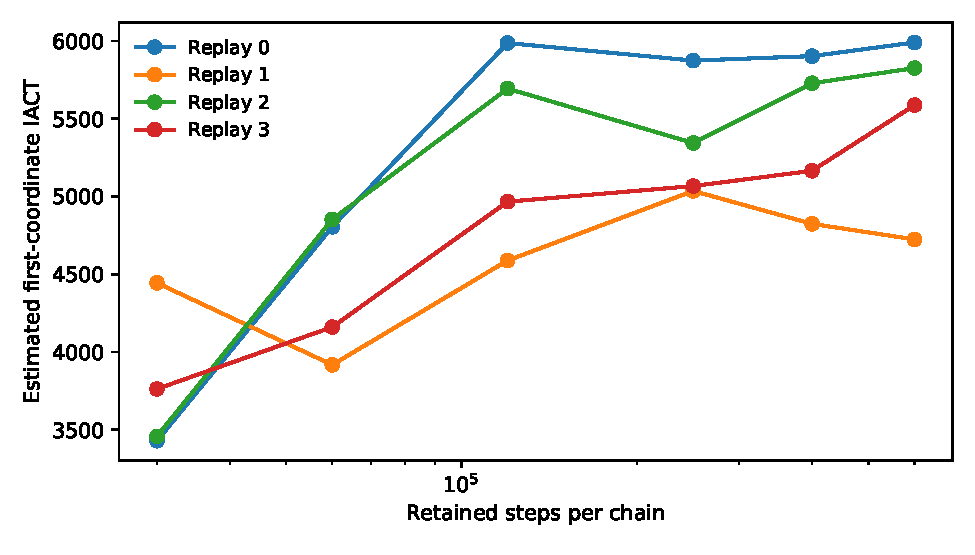
\includegraphics[width=.86\linewidth]{figures/iact_prefix_R4.pdf}
\caption{Newly re-executed prefix calculations on four historical paths. Nonflat and separated curves expose finite-run sensitivity; no final stabilization or rigorous mixing-time bound is inferred.}\label{fig:iactstability}
\end{figure}

The historical thirty-two-component scalar mixture is timed in eight new warmed blocks, using a separate fixed seed to randomize method order. Each method repeats its seed-195946 path with sixteen chains and 45,000 steps including 5,000 discarded steps. Compilation is excluded. Return-array hashes agree across repeats of each method. Raw block times and hashes are supplied; the old twelve-block summary without its original records is not used.
\begin{table}[tb]\centering
\caption{Eight new warmed timing blocks for each fixed historical scalar path. Seconds and standard deviations measure timing variability, not new Monte Carlo uncertainty or a hardware-independent complexity.}\label{tab:repeatedscalar}
\begin{tabular}{lrrrr}\toprule Correction & Mean & SD & Minimum & Maximum\\\midrule
Conditional & 0.1079 & 0.0028 & 0.1038 & 0.1132\\
Marginal & 0.7058 & 0.0458 & 0.6536 & 0.7754\\
\bottomrule\end{tabular}\end{table}
\section{Auditable full-vector posterior comparison}
\subsection{Data and shared whitening}
The main paper defines the Bayesian logistic target and its Hessian. Both designs have correlated Gaussian rows with covariance $0.8^{|j-k|}/d$, prior standard deviation $2.5$, and $n=4d$. Data seeds are $23092026+d$. The truth vector is $1.5\cos(0.7(j-1))$ and the two test rows are generated by the same archived generator before simulating binary responses. The data matrices, responses, truth, test rows, posterior mode and whitening matrix are stored in \texttt{model\_d16.npz} and \texttt{model\_d64.npz}.

Newton iterations use the analytic positive-definite Hessian with backtracking. The infinity norms of the final physical-coordinate posterior gradients are below $7\times10^{-16}$. The physical Hessian condition numbers are $27.898$ and $41.468$. After whitening, the normwise errors from the identity Hessian at the mode are below $2.5\times10^{-15}$. Global transformed Hessian eigenvalue bounds from the displayed formula are $[0.02795,1.63944]$ and $[0.01989,1.63593]$, respectively. These bounds prove strong log-concavity, not numerical equality with a Gaussian. The maximum eigenvalues of the prior precision $Q=P$ are $0.779828$ and $0.824795$; the main article's quadratic-confinement proposition applies to the auxiliary step $\tau=0.8$, with linear contraction norms $0.973605$ and $0.981218$. The identity Hessian at the mode implies $Q\preceq I$, so the simpler bound $\tau<2/c_\alpha$ also verifies the required condition without relying on numerical eigenvalue sharpness. The likelihood-plus-linear-shift gradient is globally bounded. This gives fixed-dimensional geometric ergodicity, not a uniform numerical contraction constant for the full MH kernel. Mixed off-mode Hessian entries reach $0.0558$ and $0.0380$ in independently checked points.

The common transform $\beta=\widehat\beta+Dz$ gives a transformed log density, up to a constant,
\[
 \ell(z)=-\sum_i\{\log(1+e^{a_i+B_iz})-y_i(a_i+B_iz)\}
 -\tfrac12 z^TPz-l^Tz,
\]
where $a=X\widehat\beta$, $B=XD$, $P=D^TD/2.5^2$ and $l=D^T\widehat\beta/2.5^2$. The code uses a stable log-one-plus-exponential branch and its exact analytic gradient. All models and all kernels share this evaluator. The normalizing constant is never required.

\subsection{Frozen kernels and configurations}
The active \texttt{code/samplers.py} and diagnostic modules are byte-identical to the reviewed R3 implementation. The new \texttt{benchmark\_R4.py} controls measurement and complete per-replicate recording. Invalid arithmetic aborts before state acceptance; a failed run is not silently replaced. The forty-case regression suite is rerun before this experiment.

Gaussian random walk is $z'=z+sZ$; MALA is $z'=z+s^2\nabla\ell(z)/2+sZ$ with the complete forward/reverse Gaussian ratio. Stable random walk uses $z'=z+s\xi$ and the symmetric ratio. Auxiliary and finite-mixture methods use $z'=z+c_\alpha\tau\nabla\ell(z)+\tau^{1/\alpha}\xi$, with their respective conditional or marginal corrections. The latter generates from its actual finite node distribution, not a continuous stable law. The stable index is $1.5$. The archived sixteen-node arrays in the two model files agree exactly and are used unchanged. All generation and density evaluations share the same nodes and weights.

The Laplace-reference proposal is $e^{-T}z+\sqrt{1-e^{-2T}}Z$, with $T=t$ or $t^{2/\alpha}S$, and log ratio $\ell(z')-\ell(z)+(\|z'\|^2-\|z\|^2)/2$. HMC uses identity mass, full momentum refresh, step uniform on $[0.9s,1.1s]$, and leapfrog count uniform on $\{\max(1,L-2),\ldots,L+2\}$. Finite Hamiltonian errors are Metropolis corrected; errors of absolute size above 1000 are counted separately. Nonfinite arithmetic instead stops the run.

The configurations in Table~\ref{tab:currenttuning} are inherited fixed inputs, not newly optimized choices. No pilot is run or charged. A history note records the preceding finite search without claiming its unavailable per-candidate measurements were recovered. Every configuration uses eight four-chain replicates and $N(0,I_d)$ initial states in the common Laplace coordinates, with 5,000 discarded steps. The new protocol fixes all settings, seeds, lengths, order and screening before execution. There is no extension, retuning or favorable replacement after observing results.
\begin{table}[tb]\centering\small
\caption{Frozen inputs for the newly recorded comparison. Step denotes $s$ for random walks, MALA and HMC, $\tau$ for drifted corrections, and $t$ for clocks. Nominal HMC counts have independent jitter.}\label{tab:currenttuning}
\begin{tabular}{rlrr}\toprule $d$ & Method & Step/count & Retained per chain\\\midrule
16&Gaussian RW&0.6&80\,000\\
&Gaussian MALA&0.94494&40\,000\\
&HMC&0.3, $L=5$&40\,000\\
&Stable RW&0.45&80\,000\\
&Auxiliary stable&0.8&40\,000\\
&Marginal mixture (16)&0.8&40\,000\\
&Laplace-reference pCN&4&40\,000\\
&Laplace-reference stable clock&1.5&40\,000\\
\midrule
64&Gaussian RW&0.3&200\,000\\
&Gaussian MALA&0.75&40\,000\\
&HMC&0.4, $L=3$&40\,000\\
&Stable RW&0.225&300\,000\\
&Auxiliary stable&0.8&40\,000\\
&Marginal mixture (16)&0.8&40\,000\\
&Laplace-reference pCN&4&40\,000\\
&Laplace-reference stable clock&1.5&40\,000\\
\bottomrule\end{tabular}\end{table}

\subsection{Diagnostics, recording and random streams}
Performance is the minimum bulk or tail ESS over $\beta_1,\beta_2,\beta_{d/2+1},\beta_d$, the alternating normalized contrast, two fixed predictive probabilities and $\ell(z)$. Screening additionally checks all physical coefficients, all prior-precision eigenvectors ordered by increasing eigenvalue, and eight normalized Gaussian directions from seed $45570000+d$. There are $2d+16$ quantities, transformed in small blocks without time thinning. Rank-normalized folded split-$\widehat R$, bulk ESS, 0.05/0.95 tail ESS and raw-mean ESS use the pinned \texttt{arviz-stats} interface \citep{vehtari}. Nonfinite or undefined evidence, constant chain functionals, invalid times and no movement cannot pass. Otherwise the fixed screen requires $\widehat R\le1.01$ and both ESS values at least 400 throughout. It is not a familywise test or a stationary-error certificate.

For dimension $d$, method $m=0,\ldots,7$, replicate $r=0,\ldots,7$ and chain $c=0,\ldots,3$, initial states use seed $54000000+1000d+10r+c$. Warm-up uses $55000000+10000d+1000m+10r+c$; retained sampling adds $10000000$. These existing schedules are reused, so newly measured times do not add independent accuracy evidence to the preceding runs. Method order within each replicate uses a separate seed $89000000+d+r$.

All states and eight performance quantities are recorded every retained iteration inside the timed kernel. Every diagnostic is computed before thinning. Each JSON record contains full primary and expanded diagnostics, chain means and standard deviations, acceptance/evaluation/energy-error metrics, seeds, times, and hashes of the complete unthinned arrays. Inspection files retain observations every twentieth step and states every hundredth step, together with initial, post-warm-up and final states. The supplied code and hashes permit regeneration of the full arrays. Thinned inspections are not used to recompute ESS.
\begin{table}[tb]\centering\footnotesize\setlength{\tabcolsep}{4pt}
\caption{Expanded diagnostics for the newly executed comparison. Extrema cover every replica and every declared quantity. A passing finite-run screen is not proof of mean accuracy.}\label{tab:currentdiagnostics}
\begin{tabular}{rlrrrr}\toprule $d$&Method&Failed&Max. $\widehat R$&Min. bulk&Min. tail\\\midrule
16&Gaussian RW&0/8&1.00249&4\,913&8\,787\\
&Gaussian MALA&0/8&1.00044&28\,550&35\,860\\
&HMC&0/8&1.00007&94\,407&114\,912\\
&Stable RW&0/8&1.00270&3\,667&6\,976\\
&Auxiliary stable&0/8&1.00051&22\,376&25\,853\\
&Marginal mixture (16)&0/8&1.00033&37\,195&39\,905\\
&Laplace-reference pCN&0/8&1.00030&22\,066&8\,175\\
&Laplace-reference stable clock&0/8&1.00024&24\,932&12\,384\\
\midrule
64&Gaussian RW&0/8&1.00391&2\,917&5\,986\\
&Gaussian MALA&0/8&1.00084&15\,699&27\,991\\
&HMC&0/8&1.00026&54\,150&64\,789\\
&Stable RW&0/8&1.00322&3\,712&7\,414\\
&Auxiliary stable&0/8&1.00094&10\,405&12\,948\\
&Marginal mixture (16)&0/8&1.00066&16\,777&17\,678\\
&Laplace-reference pCN&0/8&1.00073&8\,712&2\,924\\
&Laplace-reference stable clock&0/8&1.00125&6\,801&2\,863\\
\bottomrule\end{tabular}\end{table}

\subsection{Costs and aggregation}
All methods share the dense double-precision evaluator and one numerical-library thread. All used numerical and recording paths are warmed before timing. Sampling encloses the validated kernel call, including RNG initialization, current target evaluation, proposals, corrections and dense recording. Warm-up encloses the nonrecording 5,000-step call. Diagnostics include both primary and expanded calculations on unthinned arrays.

Let $E_r$ be a replicate's minimum bulk ESS over the eight performance quantities and $S_r,W_r,D_r$ its sampling, warm-up and diagnostic times. The reported rates are
\[
 R_r^{\rm sample}=E_r/S_r,\qquad R_r^{\rm assessed}=E_r/(S_r+W_r+D_r).
\]
Each table entry is the mean of replicate-specific rates, with standard error equal to their sample standard deviation divided by $\sqrt8$. The tail rate uses its own minimum ESS. We do not divide separately averaged numerators and denominators. Raw failed rates remain recorded, but a configuration with a failed replicate would be unqualified rather than ranked.

Shared setup, JIT warming, copying, hashes, compression, and JSON/summary bookkeeping are excluded. Model loading, compression, and elapsed time through the pre-JSON-write boundary are also recorded. Assessed time therefore includes the principal validation computation but is not end-to-end time or pilot-inclusive startup cost. No historical timer is imputed. These machine-specific errors condition on one data set and fixed settings; they do not cover retuning or another hardware environment. Host contention may affect short measurements despite one-thread execution and randomized method order.
\begin{table}[tb]\centering\footnotesize\setlength{\tabcolsep}{4pt}
\caption{New wall times, in seconds. Values are replicate means; sampling and warm-up sum four sequential chains. Assessed time is formed within the replica before calculating efficiency. Diagnostic costs are measured, not represented as free.}\label{tab:currentcost}
\begin{tabular}{rlrrrr}\toprule $d$&Method&Sampling&Warm-up&Diagnostics&Assessed\\\midrule
16&Gaussian RW&1.00&0.06&7.87&8.93\\
&Gaussian MALA&0.58&0.07&5.06&5.71\\
&HMC&2.30&0.28&5.30&7.88\\
&Stable RW&1.04&0.06&7.71&8.81\\
&Auxiliary stable&0.61&0.08&4.15&4.83\\
&Marginal mixture (16)&0.68&0.08&4.52&5.28\\
&Laplace-reference pCN&0.56&0.07&5.09&5.71\\
&Laplace-reference stable clock&0.57&0.07&5.14&5.78\\
\midrule
64&Gaussian RW&18.72&0.45&58.94&78.12\\
&Gaussian MALA&4.61&0.56&13.99&19.17\\
&HMC&12.62&1.56&14.66&28.84\\
&Stable RW&29.34&0.47&116.26&146.07\\
&Auxiliary stable&4.74&0.59&9.81&15.14\\
&Marginal mixture (16)&4.83&0.61&10.76&16.21\\
&Laplace-reference pCN&4.20&0.51&13.08&17.79\\
&Laplace-reference stable clock&4.34&0.53&13.59&18.46\\
\bottomrule\end{tabular}\end{table}

\subsection{Same-proposal component sensitivity}
At $d=64$, fix $\tau=0.8$ and compare marginal $M=8,16,32$ mixtures against conditional $M=16$ correction. Each row has four four-chain replicates, 5,000 discarded and 40,000 retained steps, and $N(0,I_d)$ starts. No component-specific tuning or extension is used. Nodes for $M=8,32$ are fixed positive-stable quantile midpoints; the sixteen-node law is the archived array. All actual node bytes are supplied.

Component rows add $30000000$ to the primary seed formulas and use seed-method code 5 for every row. Thus they deliberately share random streams; that coupling does not create extra independent replication. The two sixteen-node methods use the same proposal; other component counts change it. Row order uses $89500000+r$. Timing and diagnostic definitions are identical to the primary experiment. The same-proposal ordering concerns asymptotic variance, not a universal ESS/s ordering.
\begin{table}[tb]\centering\footnotesize\setlength{\tabcolsep}{4pt}
\caption{New component-sensitivity records at $d=64$. Four four-chain replicas per row; no component-specific tuning. Rates use the same eight performance functionals and the expanded screen.}\label{tab:components}
\begin{tabular}{lrrrrr}\toprule Correction&Accept.&Bulk/s&Tail/s&Assessed/s&Failed\\\midrule
Marginal, $M=8$&0.276&$4\,101\pm 44.8$&$4\,408\pm 58.9$&$1\,212\pm 15.2$&0/4\\
Marginal, $M=16$&0.277&$4\,190\pm 30.5$&$4\,390\pm 39.0$&$1\,236\pm 6.6$&0/4\\
Marginal, $M=32$&0.276&$4\,134\pm 27.7$&$4\,424\pm 102.3$&$1\,228\pm 7.1$&0/4\\
Conditional, $M=16$&0.202&$2\,391\pm 18.0$&$3\,054\pm 30.2$&$734.8\pm 6.9$&0/4\\
\bottomrule\end{tabular}\end{table}
\subsection{Preserved reference and fixed-plan uncertainty assessment}\label{sec:r3uncertainty}
The focused R3 validation remains supplied with its executed records, source and unthinned contrast traces. It is not relabeled as newly sampled reference data. The current primary run preserves the original contrast seed schedule. The archived HMC reference was replayed under the guarded modules and independently repeated in the R3 review; those operations improve traceability, not statistical independence. Prefixes and batch sizes were fixed before reconstruction, without favorable-seed search or optional extension.

\paragraph{Reference replay.}
The reference uses its original eight chains per dimension, 6,000 discarded and 80,000 retained steps, nominal step $0.35$, count five and the same independent jitter. Initial states are $2Z$ with initial seed $14200000+10d+c$; warm-up and retained seeds are $14300000+10d+c$ and $14400000+10d+c$. Across all sixteen chains, every available every-twentieth-step eight-functional observation and each of the five archived kernel metrics agree bitwise. All seven recomputed original diagnostic arrays (means, standard deviations, raw-mean errors, rank $\widehat R$, bulk/tail/mean ESS) have zero maximum difference from their archived values. R3 additionally applies the full $2d+16$-quantity screen to the unthinned reference output.

\begin{table}[!htbp]\centering\small
\caption{Expanded reference diagnostics after the original-seed replay. Minima and maxima range over the declared quantities, not only the eight performance functionals. Both rows pass the stated finite-run screen. These are the same reference paths, not new independent draws.}\label{tab:reference_r3}
\begin{tabular}{rrrrr}\toprule
$d$&Quantities&Maximum $\widehat R$&Minimum bulk ESS&Minimum tail ESS\\\midrule
16&48&1.00002187&349,349&450,671\\
64&144&1.00003489&305,486&346,176\\
\bottomrule\end{tabular}\end{table}
The reference mean of the dimension-16 contrast remains $0.957706614$, with raw-mean MCSE $0.002330954$. An expanded screen does not turn this Monte Carlo reference into ground truth. Independent physical-coordinate target calculations over 80 checks per dimension have maximum centered-log-density discrepancy $3.13\times10^{-13}$ and directional-derivative discrepancy $3.88\times10^{-9}$. A separate Python random-walk loop using a NumPy physical-coordinate target reproduces a 5,000-step common-proposal/uniform control path exactly. This tests different implementation components; it does not prove that every long-run error has been eliminated.

\paragraph{Direct comparison, without the HMC reference.}
The original and targeted-follow-up means are $0.936894$ and $0.972832$, with reported between-replicate errors $0.003316$ and $0.006213$. Their difference is approximately $0.035938$, and
\[
 \frac{0.972832-0.936894}{\sqrt{0.003316^2+0.006213^2}}=5.103\quad\hbox{(approximately)}.
\]
This descriptive ratio contains no reference error. It must not be described as a calibrated Gaussian test: the contrast was selected after a search across reported results, each group has only eight replicate means, and both error bars are estimated. The follow-up/reference ratio $2.28$ alone does not settle the original concern. All primary values and original denominators are retained.

\paragraph{Aggregation formulas.}
Let $f_{rci}$ be the contrast in group $r=1,\ldots,R$, chain $c=1,\ldots,C$, and retained time $i=1,\ldots,n$, with $R=8$ and $C=4$. Define
\[
 m_{rc}=n^{-1}\sum_i f_{rci},\qquad m_r=C^{-1}\sum_c m_{rc},
 \qquad \bar m=R^{-1}\sum_r m_r.
\]
The reported between-replicate standard error is
\[
 s_B^2=\frac{\sum_r(m_r-\bar m)^2}{R(R-1)}.
\]
For comparison, $s_C$ is the sample standard deviation of the $RC=32$ chain means divided by $\sqrt{RC}$. If $q_r$ is the four-chain raw-mean MCSE returned for replicate $r$, the previously reported within-replicate aggregation is
\[
 s_W=\frac{\sqrt{\sum_{r=1}^R q_r^2}}{R}.
\]
The division by $R$, rather than $\sqrt R$, follows from the equal-weight mean of $R$ independent replicate estimates. Bulk ESS is not used to compute $q_r$.

\begin{table}[!htbp]\centering\small
\caption{All eight full-length replicate means reconstructed from the documented seeds. The last two columns are four-chain raw-mean MCSEs, not between-replicate errors. All 64 individual chain means, including the prefix means, are in \texttt{contrast\_chains.csv}.}\label{tab:all_replicates}
\begin{tabular}{rrrrr}\toprule
Replicate&Original mean&Follow-up mean&Original $q_r$&Follow-up $q_r$\\\midrule
0&0.933572&0.964911&0.025839&0.024936\\
1&0.922512&0.964744&0.025653&0.024505\\
2&0.933306&0.968519&0.025566&0.024821\\
3&0.935580&0.972597&0.025259&0.026122\\
4&0.943425&0.981097&0.025260&0.025541\\
5&0.945790&0.962497&0.026328&0.025398\\
6&0.929631&1.012286&0.025115&0.024659\\
7&0.951340&0.956006&0.025980&0.025485\\
\bottomrule\end{tabular}\end{table}

For a nonoverlapping batch size $b$ and $a=\lfloor n/b\rfloor$, let $M_{rcj}$ be each complete batch mean. The finite-run batch-means error estimate is
\[
 \widehat v_{rc,b}=\frac{1}{a(a-1)}\sum_{j=1}^{a}(M_{rcj}-\overline M_{rc})^2,
 \qquad s_{\mathrm{BM},b}=\frac{\sqrt{\sum_{r,c}\widehat v_{rc,b}}}{RC}.
\]
This is a standard batch-means diagnostic \citep{flegal}; no finite-run consistency guarantee is inferred from the formula. Chains are never concatenated before forming batches. The fixed grid is $b\in\{50,100,200,400,800,1600,3200\}$, prefixes are $n\in\{10,000,20,000,40,000,80,000\}$, and combinations with fewer than 25 complete batches per chain are excluded. Any remainder is reported as unused in the estimator. The grid is fixed before reconstruction, not selected for a preferred denominator.

\begin{table}[!htbp]\centering\small
\caption{Full-length uncertainty sensitivity for the equal-weight average. These are alternative diagnostics, not replacements for the original $s_B$. Batch sizes omitted from this compact table remain in the CSV and figure.}\label{tab:uncertainty_r3}
\begin{tabular}{lrrrrrr}\toprule
Group&$s_B$&$s_C$&$s_W$&BM 200&BM 800&BM 3200\\\midrule
Original&0.003316&0.009320&0.009061&0.008473&0.008858&0.008751\\
Follow-up&0.006213&0.009558&0.008905&0.008307&0.008786&0.008699\\
\bottomrule\end{tabular}\end{table}
The original $s_C$ and $s_W$ are both near $0.009$, while $s_B$ is $0.003316$. Thus the grouping into eight four-chain means gives a substantially smaller error estimate in this realization. The corresponding full-length batch-means values are also much closer to $s_W$ than to the original $s_B$. This demonstrates sensitivity to variance estimation and aggregation; it does not establish which finite-run error estimate is correct, identify a stationary bias, or validate retroactive replacement of error bars. Combining the two $s_W$ values gives a direct-group standardized difference $2.829$, rather than $5.103$. Both diagnostics are reported with their original definitions.

\begin{figure}[!htbp]\centering
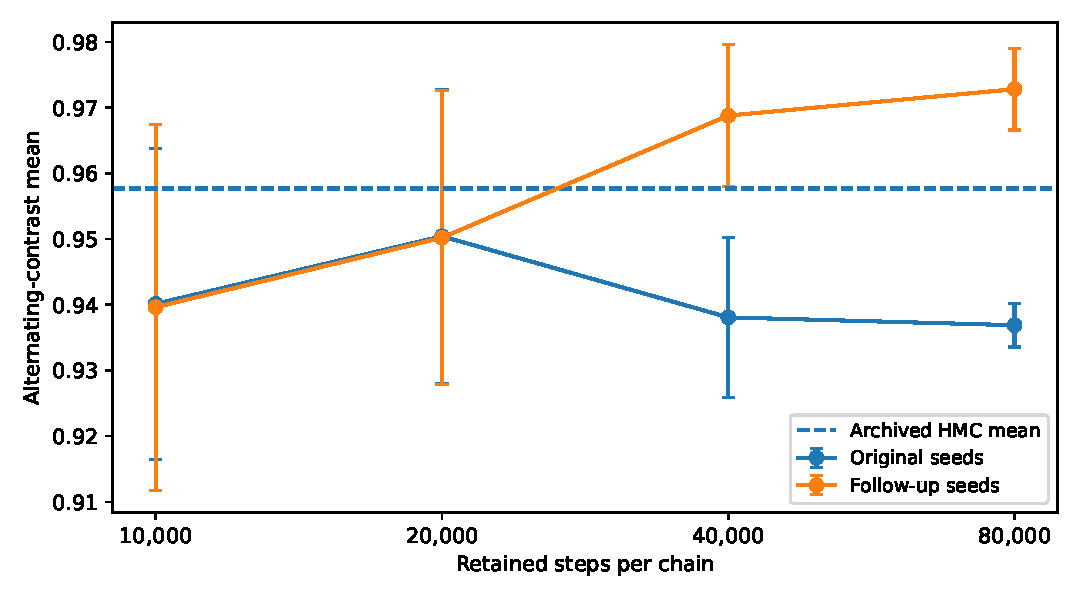
\includegraphics[width=.85\linewidth]{figures/contrast_prefix_R3.pdf}
\caption{Prefix means of the two reconstructed contrast groups with their original between-replicate standard errors. Prefixes share paths. The horizontal reference is the archived HMC mean, not an exact value. The full-length primary and follow-up values are not pooled.}\label{fig:contrast_prefix}
\end{figure}
\begin{figure}[!htbp]\centering
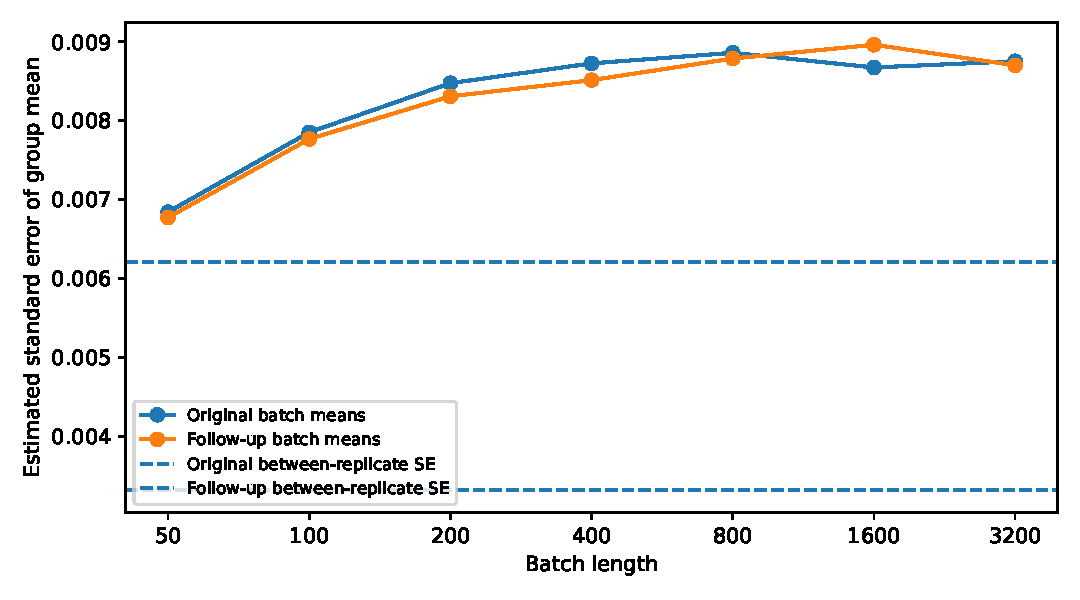
\includegraphics[width=.85\linewidth]{figures/contrast_batch_R3.pdf}
\caption{Full-length batch-means sensitivity for the group average. Horizontal lines show the originally defined between-replicate errors, not a selected correction. Dependence across batch sizes prevents treating points as independent replications.}\label{fig:contrast_batch}
\end{figure}
The uncertainty question remains open at the level of these finite runs. Exact-seed reconstruction and the separate implementation control did not expose a transition error, but passing diagnostics cannot rule out mean error or transient effects. The appropriate conclusion is exploratory throughput with an explicitly unresolved contrast, not a certified accuracy-qualified efficiency result. No new independent seed group was drawn during this revision to reduce the discrepancy.

\subsection{Dispersed-start failure details}
A fixed-plan R3 reconstruction also applies the documented $40,000,000$ study offset to the reported initial, warm-up and sampling seed formulas for the two dimension-64 Laplace-reference controls. It uses four four-chain replicates, the published clocks, 5,000 discarded and 40,000 retained steps, and $N(0,4I)$ starts. This is not a claim of byte identity to unavailable original cold-start records. Seven of the eight reconstructed replicates contain a completely frozen chain and fail with explicit constant-chain and no-move reason codes. The remaining stable-clock replicate has accepted moves in all four chains but fails the finite statistical screen (maximum $\widehat R=1.03826$, minimum bulk ESS $65.29$, minimum tail ESS $14.72$). No numerical abort occurs. Table~\ref{tab:cold_r3_counts} separates zero movement from an arithmetic failure.

\begin{table}[!htbp]\centering\small
\caption{Accepted moves in each reconstructed 40,000-step cold-start chain. All eight four-chain replicates fail the stated screen; zero means no accepted retained move, not missing data.}\label{tab:cold_r3_counts}
\begin{tabular}{llrrrr}\toprule
Method&Replicate&Chain 0&Chain 1&Chain 2&Chain 3\\\midrule
Fixed clock&0&21071 & 21247 & 4277 & 0\\
Fixed clock&1&10856 & 21703 & 0 & 15246\\
Fixed clock&2&21574 & 21168 & 0 & 21114\\
Fixed clock&3&0 & 20983 & 21555 & 2246\\
Stable clock&0&22947 & 23432 & 22793 & 0\\
Stable clock&1&18966 & 22624 & 23155 & 22735\\
Stable clock&2&22551 & 22837 & 0 & 23029\\
Stable clock&3&0 & 23017 & 23112 & 20395\\
\bottomrule\end{tabular}\end{table}

\subsection{Executable release and limits}
This supplement preserves scientific version R5 and uses the unchanged numerical release R4-frozen-1. In the accompanying repository package, \path{reproducibility/stable_score_R4_core/} contains the guarded modules, tests, exact model and node arrays, frozen protocol, every primary and component diagnostic and timer, and the independent aggregation audit. Preserved R3 reference and contrast summaries remain in its \texttt{results\_R3/} directory. The separate directory \path{reproducibility/stable_score_historical_diagnostics/} supplies the historical scripts and records identified in Table~\ref{tab:files}.

The repository-relative \texttt{ARTIFACT\_MAP.json} links every numerical table and figure to the current manuscript source and unchanged numerical records. The root checksum manifest identifies the packaged files; \texttt{RELEASE\_ASSETS.json} identifies the separately supplied optional inspection and prior-validation archives. Original numerical package manifests remain unchanged. Earlier unavailable timing summaries are preserved only as history and are not combined with the current performance records. Tests and hashes supplement rather than replace mathematical arguments.

Run the following commands from \path{reproducibility/stable_score_R4_core/} in a working copy, preserving the deposited records first. The root wrapper \texttt{scripts/run\_checks.py} instead runs audits and safety checks in a temporary copy.

The principal commands are
\begin{verbatim}
python tests/test_safety.py
python code/benchmark_R4.py run
python code/benchmark_R4.py analyze
python code/audit_R4.py
\end{verbatim}
The shipped protocol is already frozen. The driver explicitly skips completed matching records and rejects incomplete or source-mismatched records. Running it against supplied completed outputs is not a new simulation. The README gives a clean-copy procedure that preserves supplied records before independent re-execution. The audit only reaggregates records unless replay is explicitly requested. Historical prefix/timer checks require the separately supplied historical package and are executed with \texttt{additional\_R4.py}.

The fixed configurations are not claimed optimal, the posterior is not heavy-tailed or an expensive inverse solve, and the benchmark uses analytic values and gradients. The unresolved contrast remains a finite-sample limitation, not a concealed favorable-seed replacement. Permanent public archiving, contact details, factual declarations and an appropriate license remain author decisions. No external human endorsement or formal proof certificate is asserted.

\subsection*{Data and code access}
% SUPPLEMENT_AVAILABILITY_BEGIN
The author-designated repository for the source code, synthetic data and reproducibility records is
{\def\UrlBreaks{\do\/\do-\do.}\url{https://github.com/tvu25/Score-based-Metropolis--Hastings-with-stable-proposals}}. \textbf{[AUTHOR: confirm public access and specify a release tag or commit.]}
The accompanying package preserves numerical release R4-frozen-1; repository-relative instructions and an artifact map identify its records. Optional trace assets are listed with SHA256 checksums in \texttt{RELEASE\_ASSETS.json}. Truong Vu is the sole author of the article and this supplement.
% SUPPLEMENT_AVAILABILITY_END

\begin{thebibliography}{99}
\bibitem[Aloui et~al.(2026)Aloui, Liao, Hasan, Blanchet, and Tarokh]{fractional} Aloui A, Liao J, Hasan A, Blanchet J, Tarokh V (2026) \emph{Score-based Metropolis-Hastings for Fractional Langevin Algorithms}, arXiv:2602.00835v1. \url{https://arxiv.org/abs/2602.00835v1}.
\bibitem[Chambers et~al.(1976)Chambers, Mallows, and Stuck]{cms} Chambers JM, Mallows CL, Stuck BW (1976) A method for simulating stable random variables,
\emph{Journal of the American Statistical Association} 71:340--344. \url{https://doi.org/10.1080/01621459.1976.10480344}.
\bibitem[Flegal and Jones(2010)Flegal and Jones]{flegal} Flegal JM, Jones GL (2010) Batch means and spectral variance estimators in Markov chain Monte Carlo, \emph{Annals of Statistics} 38:1034--1070. \url{https://doi.org/10.1214/09-AOS735}.
\bibitem[Geyer(1992)Geyer]{geyer} Geyer CJ (1992) Practical Markov chain Monte Carlo,
\emph{Statistical Science} 7:473--483. \url{https://doi.org/10.1214/ss/1177011137}.
\bibitem[Kanter(1975)Kanter]{kanter} Kanter M (1975) Stable densities under change of scale and total variation inequalities,
\emph{Annals of Probability} 3:697--707. \url{https://doi.org/10.1214/aop/1176996309}.
\bibitem[Sj\"oberg et~al.(2026)Sj\"oberg, Lindqvist, \"Onnheim, Jirstrand, and Svensson]{sjoberg} Sj\"oberg A, Lindqvist J, \"Onnheim M, Jirstrand M, Svensson L (2026) MCMC-correction of score-based diffusion models for model composition,
\emph{Entropy} 28:article 351. \url{https://doi.org/10.3390/e28030351}. Preprint first submitted as arXiv:2307.14012 in 2023.
\bibitem[Vehtari et~al.(2021)Vehtari, Gelman, Simpson, Carpenter, and B\"urkner]{vehtari} Vehtari A, Gelman A, Simpson D, Carpenter B, B\"urkner P-C (2021) Rank-normalization, folding, and localization: an improved $\widehat R$ for assessing convergence of MCMC (with discussion), \emph{Bayesian Analysis} 16:667--718. \url{https://doi.org/10.1214/20-BA1221}.
\end{thebibliography}
\end{document}
